\documentclass{amsart}

\newtheorem{theorem}{Theorem}[section]
\newtheorem{lemma}[theorem]{Lemma}

\theoremstyle{definition}
\newtheorem{definition}[theorem]{Definition}
\newtheorem{example}[theorem]{Example}
\newtheorem{xca}[theorem]{Exercise}

\theoremstyle{remark}
\newtheorem{remark}[theorem]{Remark}

\numberwithin{equation}{section}

% Some packages
\usepackage{listings, color, keyval}

% Some commands
\newcommand{\RR}{\mathbb{R}}
\newcommand{\NN}{\mathbb{N}}
\newcommand{\CC}{\mathbb{C}}
\newcommand{\II}{\mathbb{I}}
\newcommand{\KK}{\mathbb{K}}


%%% Florian
\usepackage[foot]{amsaddr}
\newcommand{\Id}{\mathrm{I}}
\renewcommand{\vec}{\textbf}
\usepackage{graphicx}
\usepackage[left=2cm,right=2cm,top=2.6cm,bottom=1.4cm,includefoot]{geometry}
\usepackage[hidelinks]{hyperref}
\setcounter{tocdepth}{1}    % entries down to \sections in the TOC
\newcommand{\norm}[1]{\left\lVert#1\right\rVert}



\begin{document}

\title{Iterative Methods}

%author information
\author{Thanh-Van Huynh, Michael Thiele, Florian Wolf}
\email{thanh-van.huynh@uni-konstanz.de, michael.thiele@uni-konstanz.de, florian.2.wolf@uni-konstanz.de}
\date{\today}

\dedicatory{Thanks Gabriele and Christian for your great work.}

\begin{abstract}
This is a report about the findings of Thanh-Van Huynh, Michael Thiele and Florian Wolf in the exercises accompanying Iterative Methods for Linear Systems. The lecture was held by Jun.-Prof. Dr. Gabriele Ciaramella with the assistance of Christian J\"ackle in the winter term 2020/21 at the University of Constance.
\end{abstract}

\maketitle

\tableofcontents


%% ====================================================================

\section{Introduction}
In the exercises we studied optimal control problems governed by the Laplace equation. We want to solve
\begin{align}
\min\limits_{y,u\in L^2(\Omega)} J(y,u) &:= \frac{1}{2}\ \norm{y-y_d}
_{L^2(\Omega)}^2 + \frac{\nu}{2}\ \norm{u}_{L^2(\Omega)}^2\\
\text{s.t. } -\Delta y &= f+ u \text{ in } \Omega\\
y &= 0 \text{ on } \partial\Omega
\end{align}
for a regularization parameter $\nu > 0$. We are looking for a control function $u$. With discretized norm
\begin{equation*}
\norm{\vec{x}}_{L_h^2(\Omega)}^2 := h^2 \sum\limits_{j=1}^n \vec{x}_j^2
\end{equation*}
for $h>0$ small enough, such that
\begin{equation*}
A\vec{y}=\vec{f}+\vec{u}
\end{equation*}
is satisfied. Here $A = -\frac{1}{h^2}\cdot T$ where $T$ is the two-dimensional laplace matrix, as we will see later. Notice that we do not have any boundary conditions. One possible way of finding a solution is the so-called reduced approach: We consider $\vec{y}$ as a function of $\vec{u}$, therefore obtaining the problem
\begin{equation*}
\min\limits_{\vec{u}\in\Omega} \hat{J}(\vec{u}) := J(\vec{y}(\vec{u}),\vec{u}).
\end{equation*}


%% ====================================================================
%% ====================================================================
%% ====================================================================

%% ====================================================================

\section{Stationary Methods}
\subsection{Deriving the Optimality System}
We see that
\begin{equation*}
\norm{\vec{x}}_{L_h^2(\Omega)}^2 = h^2\ \norm{\vec{x}}_2^2
\end{equation*}
holds for arbitrary $x$. In combination with $\vec{y}=A^{-1}\left(\vec{f}+\vec{u}\right)$, we obtain
\begin{flalign*}
\min\limits_{\vec{u}\in\Omega} \hat{J}(\vec{u}) 
&=\ \frac{1}{2}\ h^2 \norm{A^{-1}\left(\vec{f}+\vec{u}\right)-\vec{y}_d}_2^2\ + \frac{\nu}{2}\ h^2 \norm{\vec{u}}_2^2\\
& =\ \frac{1}{2}\ h^2 \langle A^{-1}\left(\vec{f}+\vec{u}\right)-\vec{y}_d,A^{-1}\left(\vec{f}+\vec{u}\right)-\vec{y}_d\rangle + \frac{\nu}{2}\ h^2 \langle\vec{u},\vec{u}\rangle\\
& =\ \frac{1}{2}\ h^2  \left(A^{-1}\left(\vec{f}+\vec{u}\right)-\vec{y}_d\right)^{\top} \left(A^{-1}\left(\vec{f}+\vec{u}\right)-\vec{y}_d\right) + \frac{\nu}{2}\ h^2 \vec{u}^{\top}\vec{u}.
\end{flalign*}
As we know that a solution $\vec{u}$ to the problem above has to satisfy $\nabla\hat{J}(\vec{u})=0$, this results in
\begin{equation*}
\nabla \hat{J}(\vec{u}) = h^2 A^{-1} \left(A^{-1} (\vec{f}+\vec{u})-\vec{y}_d\right) + \nu h^2\vec{u} = 0.
\end{equation*}
We can do the following transformations
\begin{flalign*}
h^2 A^{-1} \left(A^{-1} (\vec{f}+\vec{u})-\vec{y}_d\right) + \nu h^2\vec{u} &= 0\\
A^{-1} \left(A^{-1} (\vec{f}+\vec{u})-\vec{y}_d\right) + \nu \vec{u} &=0\\
A^{-1} A^{-1} (\vec{f}+\vec{u})-A^{-1}\vec{y}_d + \nu \vec{u} &=0\\
A^{-1} A^{-1} \vec{f}+A^{-1} A^{-1}\vec{u}-A^{-1}\vec{y}_d + \nu \vec{u} &=0\\
A^{-1} A^{-1} \vec{u} + \nu \vec{u} &=A^{-1}\vec{y}_d-A^{-1} A^{-1}\vec{f}\\
\left(\nu\text{I}+A^{-1} A^{-1}\right) \vec{u} &=A^{-1}\left(\vec{y}_d-A^{-1}\vec{f}\right)
\end{flalign*}
and derive the optimality system, in the report called initial system,
\begin{equation}
\left(\nu\text{I}+A^{-2}\right) \vec{u} =A^{-1}\left(\vec{y}_d-A^{-1}\vec{f}\right) \label{eq:normalOptimalitySystem}
\end{equation}1
or alternatively, in the following called factored system,
\begin{equation}
\left(A^2\nu+\text{I}\right) \vec{u} =A\vec{y}_d-\vec{f}. \label{eq:factoredOptimalitySystem}
\end{equation}


%% ====================================================================



\subsection{Laplace Matrices}
First, we implement a function \texttt{FD\_Laplacian} to create the Finite Difference matrix representation of the Laplace operator in sparse.
Depending on whether we choose $d=1$ or $d=2$, we obtain the 1D Laplace Matrix 
$$ T_1 = 
\begin{pmatrix}
-2 & 1 & & & \\
1 & -2 & 1 & & \\
& \ddots & \ddots & \ddots & \\
%& & \ddots & \ddots & 1 \\
%& & & 1 & -2  
\end{pmatrix} \in\RR^{m\times m}
$$
or the 2D Laplace Matrix (by using the Kronecker product $\otimes$)
$$ T_2 = \text{I}_m \otimes T_1 + T_1 \otimes \text{I}_m= 
\begin{pmatrix}
T_1 & \text{I}_m & & \\
\text{I}_m & T_1 & \text{I}_m & \\
& \ddots & \ddots & \ddots
\end{pmatrix} \in\RR^{m^2\times m^2}.
$$

\begin{lstlisting}[mathescape, language=Pascal, title=FD\_Laplacian,
frame=single, numbers=left, numberstyle=\tiny, tabsize=2,
morekeywords={Enter, Return, elif}, deletekeywords={of,or}, keywordstyle=\bfseries]{}
Enter: matrix dimension $m\in\NN$, $d=\{1,2\}$ choosing 1D or 2D
Return: Laplace matrix $T\in\RR^{m\times m}$
diag = -2*sparse.identity($m$)
onesUpper = sparse.eye($m,k=1$)
onesLower = sparse.eye($m,k=-1$)
$T$ = diag + onesUpper + onesLower
if $d==2$:
	eye = sparse.eye($m$)
	$T$ = sparse.kron(eye,$T$) + sparse.kron($T$,eye)
return($T$)
\end{lstlisting}

%% ====================================================================

\subsection{Fast Poisson Solver}
Now, we implement the Fast Poisson Solver \texttt{Fast\_Poisson} to efficiently solve a linear system $Au=b$. As we do not have any boundary conditions, we have a simpler implementation:

\begin{lstlisting}[mathescape, language=Pascal, title=Fast\_Poisson,
frame=single, numbers=left, numberstyle=\tiny, tabsize=2,
morekeywords={Enter, Return, elif}, deletekeywords={of}, keywordstyle=\bfseries]{}
Enter: matrix $V$ of eigenvectors of the matrix $A\in\RR^{m\times m}$, 
vector $\lambda$ of eigenvalues of the matrix $A$, 
right-hand side $b$ of the linear system
Return: solution $u$ of the linear system $Au=b$
$B$ = reshape($b,(m,m)$)
$\tilde{B} = (V^{\top}(V^{\top}B)^{\top})^{\top}$
for i in 0:m
	for j in 0:m
			$\tilde{u}_{ij}=(\tilde{B}_{i,j})/(\lambda_i+\lambda_j)$
$U = (V(V\tilde{U})^{\top})^{\top}$
$u$ = reshape($U,m^2$)
return($u$)
\end{lstlisting}

%% ====================================================================

\subsection{Convergence Analysis}
\label{seq:ConvergenceAnalysis}
Now, we solve the system (\ref{eq:normalOptimalitySystem}) by the stationary iteration
\begin{equation}
\vec{u}^{n+1} = -\frac{1}{\nu} A^{-2}\vec{u}^n + \frac{1}{\nu} A^{-1} (\vec{y}_d-A^{-1}\vec{f})
\end{equation}
and analyze its convergence behavior for different $m$ and $\nu$. First, we fix $\nu=0.01$, then $m=15$.

\begin{figure}[h!]
	\centering
	\includegraphics[scale=1.7]{./imgs/convergence_stationary}
	\caption{Convergence behaviour of the stationary iteration for different values of $m$ and $\nu$}
\end{figure}

As the figure shows, large $m$ will lead to fast convergence. The same goes for $\nu$: bigger values are the key to convergence, while choosing small $\nu$ will result in divergence.

%% ====================================================================

\subsubsection{Eigenvectors and eigenvalues of the laplace matrices}
As we have seen in the section regarding the stationary solver and we will see this again, if we consider solving \eqref{eq:normalOptimalitySystem} 
using the conjugated gradient method, the poisson solver is the key, to get a fast solution to the $A^{-1}$ problem. The solver requires a decomposition
of the matrix $V$ in diagonalized form. In the beginning we achieved this task using \texttt{scipy.sparse.eigs}. Luckily the eigenvectors and eigenvalues
of the one dimensional laplace matrix are easy to calculate by hand, exploiting its Toeplitz-structure. For the $m\times m$ one-dimensional laplace, we 
get the following eigenvalues
\begin{align*}
\lambda_k = -2 + 2 \cos \left( \frac{\pi k}{n+1} \right), \quad k=1,\ldots, m
\end{align*} 
and the corresponding eigenvectors with entries
\begin{align*}
(\vec{v}_k)_i = \sin\left(\frac{i\cdot \pi k}{m+1} \right), \quad i,k=1,\ldots,m
\end{align*}
Now we can include these manually to get a more exact and especially quicker solver.

To get the eigenvectors and eigenvalues of the two-dimensional laplace matrix, we use problem 10 of the 
stationary iterative methods chapter of the script and proof its third bullet 
point. Therefore we use the formula $(A \otimes B)(C \otimes D) = (AC) \otimes (BD)$. For $j,k \in \{1, \ldots, m\}$ arbitrary we get for $\lambda := 
\lambda_j + \lambda_k$ and $\vec{v} := \vec{v}_j \otimes \vec{v}_k$ that
\begin{align*}
A\vec{v} &= \left(\text{I}_m \otimes T_1 + T_1 \otimes \text{I}_m \right) \vec{v}\\
&= \left( \text{I}_m \otimes T_1\right)\left(\vec{v}_j \otimes \vec{v}_k\right) + \left( T_1 \otimes \text{I}_m\right)\left(\vec{v}_j \otimes \vec{v}_k\right)\\
&= \left( \vec{v}_j \otimes \lambda_k \vec{v}_k\right) + \left( \lambda_j\vec{v}_j \otimes  \vec{v}_k\right)\\
&= \lambda_k\left( \vec{v}_j \otimes  \vec{v}_k\right) + \lambda_j\left( \vec{v}_j \otimes  \vec{v}_k\right)\\
&= \lambda \vec{v}
\end{align*}
Therefore the eigenvectors and eigenvalues of the two-dimensional laplace are obtained by using the kronecker product of the one-dimensional eigenvectors
and summing up the one-dimensional eigenvalues. We will use the eigenvalues, to calculate the condition number of the matrix in the section
about Krylov methods.

%% ====================================================================

\subsection{Damped Jacobi}
\label{sec:DampedJacobi}
Now we solve the system
\begin{equation}
(\nu A^2+ I) \vec{u} = A(\vec{y}_d-A^{-1}\vec{f}) = A\vec{y}_d-\vec{f}
\end{equation}
using the damped-Jacobi iteration
\begin{equation}
\vec{u}^{k+1} = \vec{u}^k + \omega D^{-1}\left(A \vec{y}_d-\vec{f}-(\nu A^2 + I)\vec{u}^k\right)
\end{equation}
with a damping parameter $\omega\in(0,1]$ and $D=\text{diag}(\nu A^2+I)$. Out of the three parameters $\omega=0.6, \nu=10^{-5}$ and $m=15$ we fix two and modify one in order to analyse the convergence behavior of th damped-Jacobi iteration.\\ \\
\begin{figure}[h!]
	\centering
	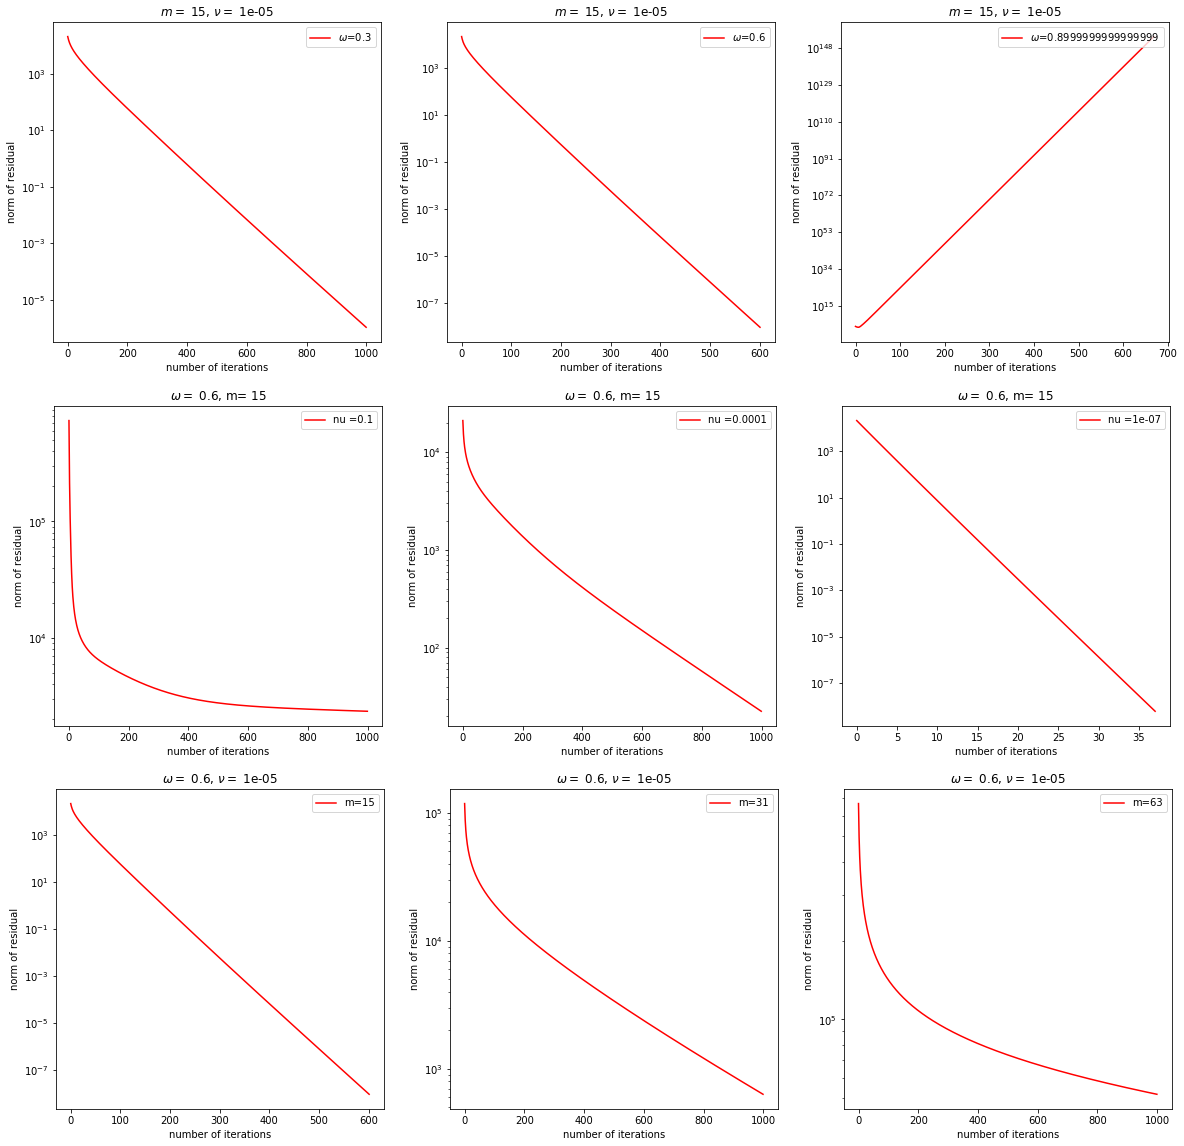
\includegraphics[scale=1.54]{./imgs/convergence_damped_jac}
	\caption{Convergence behaviour of the damped-Jacobi iteration for different values of $\omega,\nu$ and $m$}
\end{figure}
As the  figure at the bottom shows, and after some trial-and-error, we observe that $\omega\approx0.5$ is the optimal choice to reach efficient convergence. For smaller $\omega$ damped-Jacobi still converges, but slower, and for $\omega\geq0.7$ we do not obtain convergence. The dimension of $\nu$ also has a great impact: as $\nu$ gets smaller, we start to converge. As for the value of $m$, choosing bigger $m$ will lead to divergence of the damped-Jacobi method.

%% ====================================================================

\newpage
\section{Krylov Methods}

%% ====================================================================

\subsection{Convergence Analysis}
In this part of the project we want to use the fact, that the matrix arising in our disretization is symmetric and positive definite. For this reason we 
want to apply the conjugated gradient (CG) method, to solve our systems \eqref{eq:normalOptimalitySystem} and \eqref{eq:factoredOptimalitySystem}.
For the first system we use the already implemented fast poisson solver, to get a matrix free version of the left-hand side. In the second case we 
construct our sparse matrices and use the \texttt{scipy.sparse.linalg.LinearOperator} method, to create a linear operator of our left-hand side of the 
equation. So in both cases the solution process is completely matrix-free.


Looking at figure \ref{fig:CG-convergence-factored} and \ref{fig:CG-convergence-initial}, we can see the  convergence behaviour of the two systems. In the plots $\nu$ ist getting bigger going from top to bottom and $m$ is getting bigger going from left to right.
\begin{figure}[h!]
\centering
\includegraphics[scale=0.52]{./imgs/CG_analysis_factored}
\caption{Convergence behaviour for different values of $m$ and $\nu$ using CG to solve the factored systems.
The x-axis is representing the number of iterations and the y-axis shows the normalized norm of the residuals in the discretized norm.}
\label{fig:CG-convergence-factored}
\end{figure}
As you can directly see in the plots, the solution process of the factored system is getting worse, as the size of the matrix increases. The initial
system seems to be quite stable regarding finer grids. Meanwhile, the behaviour  regarding different values of $\nu$ is more interesting. While the 
convergence solving the factored system is getting worse if 
$\nu$ increases, the convergence rate of the initial system is getting faster and faster. So the systems behave in an opposite way, regarding the size of 
$\nu$.

\begin{figure}[h!]
\centering
\includegraphics[scale=0.52]{./imgs/CG_analysis_initial}
\caption{Convergence behaviour for different values of $m$ and $\nu$ using CG to solve the initial systems.
The x-axis is representing the number of iterations and the y-axis shows the normalized norm of the residuals in the discretized norm.}
\label{fig:CG-convergence-initial}
\end{figure}

%% ====================================================================

\subsection{Condition Number}
One can explain this, if we take a closer look at the conditon number of the systems for the upper combinations of $\nu$ and $m$. We can see this in 
figure \ref{fig:CG-conditionNumber-factored} and \ref{fig:CG-conditionNumber-initial}.
\begin{figure}[h!]
\centering
\includegraphics[scale=0.5]{./imgs/CG_conditionNumber_factored}
\caption{Condition numbers of the factored system for different values of $m$ and $\nu$ represented in a double-logarithmic plot.}
\label{fig:CG-conditionNumber-factored}
\end{figure}
The three plots of the condition number explain really good, why we get the upper type of convergence behaviour. While both condition numbers get overall
bigger from left to right (so with increasing matrix size due to bigger $m$), one can clearly see in each of the plots that the systems have opposed 
curves.

\begin{figure}[h!]
\centering
\includegraphics[scale=0.5]{./imgs/CG_conditionNumber_initial}
\caption{Condition numbers of the initial system for different values of $m$ and $\nu$ represented in a double-logarithmic plot. (We used small little 
crosses to indicate that the three plots overlay.)}
\label{fig:CG-conditionNumber-initial}
\end{figure}

While the factored system \eqref{eq:factoredOptimalitySystem} is worse conditioned for bigger $\nu$, the condition number of the initial system 
gets better the bigger $\nu$ is. Looking at the formulas \eqref{eq:normalOptimalitySystem} and \eqref{eq:factoredOptimalitySystem} this should now be 
really obvious.
In \eqref{eq:factoredOptimalitySystem} we factor our matrix $A^2$ by $\nu$, so the bigger $\nu$ is, the worse the condition number gets. In the initial 
system \eqref{eq:normalOptimalitySystem} the identity matrix with factor $\nu$ dominates the diagonal of the left-hand side for bigger $\nu$. So the 
condition number is getting better as $\nu$ increases, as the system is getting more and more diagonal dominant.

%% ====================================================================

\section{Multigrid}

%% ====================================================================

In our last section we use multigrid methods to solve our problems \eqref{eq:normalOptimalitySystem} and \ref{eq:factoredOptimalitySystem}. These problems can be derived by discretization, as shown in the introduction. So we are able to apply multigrid methods. We have already seen two stationary iterations:
\begin{equation}
\vec{u}^{n+1}    = - \frac{1}{\nu} A^{-2} \vec{u}^n+ \vec{f}
\label{eq: stationaryMethod}
\end{equation}
and 
\begin{equation}
\vec{u}^{n+1}    =  \vec{u}^n+ \omega D^{-1}  (\vec{f} - (\nu \Id + A^2) \vec{u}^n)
\label{eq: dampedJacobi}
\end{equation}
In the following we will refer to \eqref{eq: stationaryMethod} as the stationary method, in order to distinguish this method from \eqref{eq: 
dampedJacobi}, which is called damped Jacobi method with damping parameter $\omega \in (0,1] $. We used \eqref{eq: stationaryMethod} to solve  
\eqref{eq:normalOptimalitySystem} and \eqref{eq: dampedJacobi} to solve \eqref{eq:factoredOptimalitySystem}. Now we want to apply \eqref{eq: 
stationaryMethod} and \eqref{eq: dampedJacobi} as smoothers in a multigrid method. In both multigrid methods we use the interpolation matrix $P
$ and the full weighting restriction matrix $R:= \frac{1}{2} P^T$  in our coarse correction step. Furthermore we do one Pre-Smoothing and one Post-Smoothing step. Notice that we use the galerkin approach for our coarser matrix:
\begin{equation}
	C_{H}= R \cdot C \cdot P
\end{equation}
where $C$ is our system. It can be $\nu \Id +A^{-2}$ in the first case an in the second one $\Id +\nu A^2$, where $A$ is the Laplacian matrix divided by the grid size $h^2$. Using instead a $C_H$, which arises by a smaller grid leads to non-convergence! 
%% ====================================================================

\subsection{Stationary Methods as Smoother}
First we analyse \eqref{eq: stationaryMethod} and it's corresponding multigrid method. We expect that the convergence of our multigrid methods 
gets better for rising $\nu$. Regarding the notation of the script $M^{-1} N = - \frac{1}{\nu} A^{-2} $ is the iteration matrix of the 
stationary method. Therefore our stationary method converges faster for $\nu $ rising, which is shown in \ref{sec:DampedJacobi}. For smaller $
\nu$ we can expect slower or not even convergence at all, if the stationary method does not converge. 


\begin{figure}[h!]
	\centering
	\includegraphics[scale=0.4]{./imgs/multigrid_stat_comparison_tiny}
	\caption{Number of iterations of multigrid in comparison with the stationary method for different $\nu$ and $m$}
	\label{fig: multigridStationary}
\end{figure}
Now let us check, if our predictions were right. From figure \ref{fig: multigridStationary} we can observe, that our multigrid method even converges for small $\nu $. This can be explained by the fact, that our sationary method converges still converges for small $\nu$'s. Although we can't expect this behaviour continuing for $\nu$ decreasing. Moreover we can observe, that our method gets faster $\nu$ rising. So for very big $\nu$ the term $\nu 
\Id$ dominates $\nu \Id + A^{-2}$ and we get a iteration which would be similar to a jacobi one. Furthermore we can see that our method converges extremly quick for our selection of $\nu$'s. It needs only two to five iterations, which is enormous regarding the independecy of the mesh size. This quality can be observed in nearly every row. Additionally we can observe that our method needs for our smal $\nu$'s only a few iterations more that for our big $\nu$'s. 
In order to explain this kind of indepndency in $\nu$, we take a look at one low-frequency mode and monitor what happens, if we change $\nu$. Recalling our iteration matrix:
\begin{equation}
M^{-1}N = \frac{1}{\nu} A^{-2}
\end{equation}
we set $m=31$ and sort the eigenvalues by their absolute value in descending order. For the low frequency modes we choose the 10-th eigenvalue and the corresponding eigenvector as a representive of the low frequency modes. Now changing $\nu$ we obtain:
\begin{figure}[h!]
	\includegraphics[scale=0.4]{./imgs/10_eigenvector_of_stat_nu_001}
	\caption{10'th eigenvector of the given stationary method iteration matrix}
	\label{fig:001_ev_stat}
\end{figure}
\begin{figure}[h!]
	\includegraphics[scale=0.4]{./imgs/10_eigenvector_of_stat_nu_1}
	\caption{10'th eigenvector of the given stationary method iteration matrix}
	\label{fig:1_ev_stat}
\end{figure}
\begin{figure}[h!]
	\includegraphics[scale=0.4]{./imgs/10_eigenvector_of_stat_nu_100}
	\caption{10'th eigenvector of the given stationary method iteration matrix}
	\label{fig:100_ev_stat}
\end{figure}

From these pictures we get, that there are huge differences in the absolute values of the eigenvectors. As a result $\nu$ highly determines, whether the stationary method converges or not, but this is already explained in section \ref{seq:ConvergenceAnalysis}. The second courius fact regards the plot of the eigenvectors. The plots of the different eigenvectors are pretty similar, although $\nu$ is changing. As a consequence we can interpoline these eigenvectors on a coarser grid, still for small $\nu$. Therefore our coarse correction step produces a very good corection. This explains the small differences of iterations steps in our multigrid method, though changing $\nu$.
%% ====================================================================

\subsection{Damped Jacobi as Smoother}
Now we want to analyse the multigrid method with damped jacobi as smoother. We set $\omega= \frac{2}{3}$, so we use the optimal $\omega$ for the Laplace eqution. Let's 
make some predictions what happens, if we run our multigrid method. First we expect, that the multigrid method will be faster for shrinking $
\nu$ and slower for bigger $\nu$. Because of $I + \nu A^2$ is diagonal dominant for small $\nu$, and Jacobi converges for such systems. For 
rising $\nu$, we'll lose this effect. Nevertheless, $A^2$ is block tridiagonal:
\begin{align*}
A^2 &= (I \otimes T + T \otimes I)^2 \\
&= 2  \cdot T \otimes T + T^2 \otimes \Id + \Id \otimes T^2 
\end{align*}
That's why Jacobi should still produces reasonable results. 
\begin{figure}[h!]
	\centering
	\includegraphics[scale=0.4]{./imgs/multigrid_jac_comparison_tiny}
	\caption{Number of iterations of multigrid in comparison with damped jacobi for different $\nu$ and $m$}
	\label{fig: multigridJacobi}
\end{figure}

Again let's verify our predictions. In figure \ref{fig: multigridJacobi} we can see exactly, what we expected. Our method is great for solving 
problems with small $\nu$. Though for very small $\nu$ we come close to:
\[
\Id   \vec{v} = \vec{f}
\] 
and the solution isn't so meaningful.
Moreover we can see, that the multigrid method converges slower for $\nu$ rising.So thats again, what we predicted. But we didn't expect our method getting slower to such an extend. Notice that the multigrid method really shows it's worth in the independency we observe in every row.
In the next lines we'll take a look at one low mode from our jacobi iteration matrix  :
\begin{equation}
	M^{-1}N= \omega D^{-1}  (\frac{1}{\omega } D (\Id + \nu A^2))
\end{equation}
and observe what hapenns, if we change $\nu$. Then we can explain the phenomenon of our method loosing speed while $\nu$ increases.In the following we use $\omega=\frac{2}{3}$, $m=31$  and we obtain these eigenvectors: \par
\begin{figure}[h!]
	\includegraphics[scale=0.4]{./imgs/5_eigenvector_of_jac_nu_001}
	\caption{5'th eigenvector of damped jacobi iteration matrix}
	\label{fig:001_ev}
\end{figure}
\begin{figure}[h!]
	\includegraphics[scale=0.4]{./imgs/5_eigenvector_of_jac_nu_1}
	\caption{5'th eigenvector of damped jacobi iteration matrix}
	\label{fig:1_ev}
\end{figure}
\begin{figure}[h!]
	\includegraphics[scale=0.4]{./imgs/5_eigenvector_of_jac_nu_100}
	\caption{5'th eigenvector of damped jacobi iteration matrix}
	\label{fig:100_ev}
\end{figure}
Notice again we sorted the absolute eigenvalues from highest to lowest and choose the 5'th eigenvector as a representive of the low frequncy eigenvectors. Now from our figures \ref*{fig:001_ev},\ref*{fig:1_ev} and \ref*{fig:100_ev} we can obtain, that the corresponding eigenvalues of our eigenvectors grow. That's why convergence for damped jacobi isn't guaranteed for every $\nu$. But this finding is presented in \ref*{sec:DampedJacobi}. However the growth in comparison to the growth of $\nu$ is still very small in comparison to the growth in our first multigrid method. Now the most interesting result provides the plot of the eigenvector. For a very small $\nu$ our eigenvetor looks realy smooth, see \ref*{fig:001_ev}. So our restriction matrix can interpoline this eigenvector pretty well on a coarser grid. Thus our coarse correction step should be able to produce a strong correction. However for $\nu$ rising the eigenvector gets angular. Therefore it shouldn't be possible to interpoline the eigenvectors \ref*{fig:1_ev},\ref*{fig:100_ev} easily. This effect along with damped jacobi getting slower for rising $\nu$ explains, why our damped jacobi multigrid method gets significantly slower for rising $\nu$. 
\end{document}
